\documentclass[tikz, border=3mm]{standalone}
\usepackage{tikz}
\usetikzlibrary{arrows.meta, decorations.markings, calc}

\begin{document}
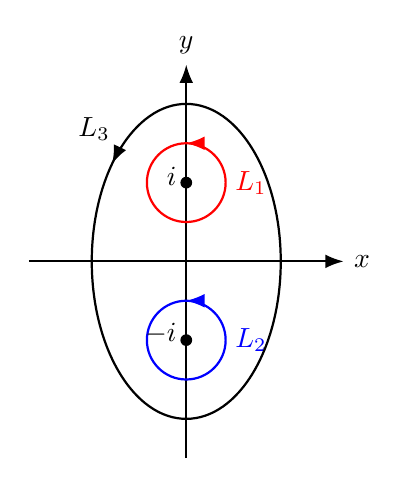
\begin{tikzpicture}[
    >=Latex, % Set default arrow tip style
    dot/.style={fill=black, circle, inner sep=1.5pt} % Style for center points
]

% Axes
\draw[->, thick] (-2, 0) -- (2, 0) node[right] {$x$};
\draw[->, thick] (0, -2.5) -- (0, 2.5) node[above] {$y$};

% Define coordinates and radii
\coordinate (c1) at (0, 1);  % Center for L1 at i
\coordinate (c2) at (0, -1); % Center for L2 at -i
\def\smallradius{0.5} % Radius for L1 and L2
\def\xradL3{1.2}      % x-radius for L3
\def\yradL3{2.0}      % y-radius for L3
\def\arrowpos{0.25}   % Arrow position (0.25 = top)

% L1 (Red, Counter-Clockwise)
\draw[red, thick,
    postaction={decorate, decoration={markings, mark=at position \arrowpos with {\arrow{>}}}}
] (c1) circle (\smallradius);
\node[red, right] at ($(c1)+(\smallradius,0)$) {$L_1$};
\node[dot, label={[left]$i$}] at (c1) {}; % Center point and label

% L2 (Blue, Clockwise)
\draw[blue, thick,
    postaction={decorate, decoration={markings, mark=at position \arrowpos with {\arrow{>}}}}
] (c2) circle (\smallradius);
\node[blue, right] at ($(c2)+(\smallradius,0)$) {$L_2$};
\node[dot, label={[left]$-i$}] at (c2) {}; % Center point and label

% L3 (Black, Counter-Clockwise)
\draw[black, thick,
    postaction={decorate, decoration={markings, mark=at position 0.375 with {\arrow{>}}}} % 0.375 is approx top-left
] (0,0) ellipse [x radius=\xradL3, y radius=\yradL3];
% Position label L3 near the arrow
\node[black, above left] at ($(0,0)+({135}:\xradL3 and \yradL3)$) {$L_3$};

% Optional: Add "Therefore" text if needed (commented out)
% \node[blue] at (1.5, -2.2) {Therefore};

\end{tikzpicture}
\end{document}